
\section{Application 1: Expression Flow for 3D-Aware Face
Component Transfer}
We now introduce one application of face fitting. The goal of this application is to transfer the mouth from one to another. We first introduce the pipeline of this project and then introduce each components in more detail.
\begin{figure}[H]
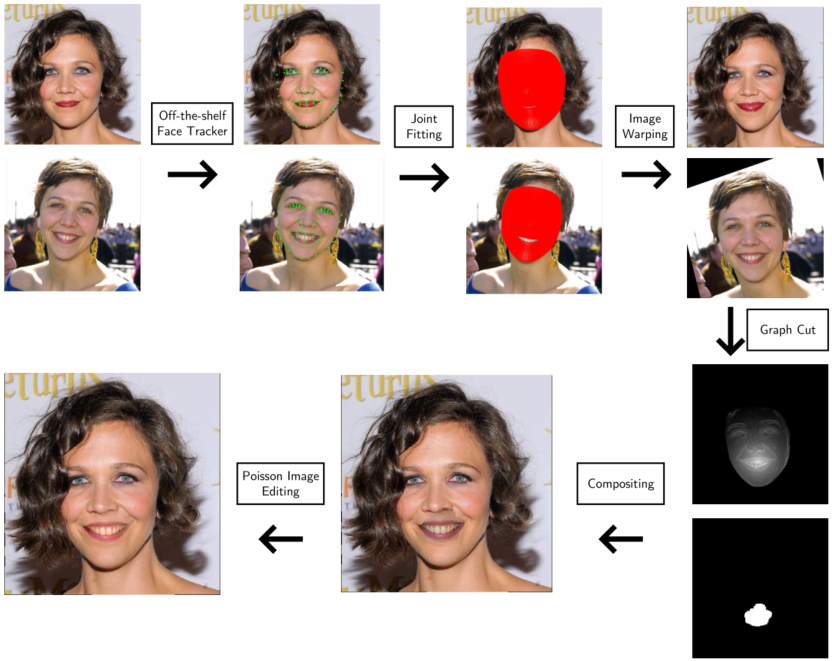
\includegraphics[width=\textwidth]{./img/expression-flow-pipeline}
\caption{Step 1: use the off-the-shelf face tracker to get the 2D face landmarks. \\
Step 2: Perform joint face fitting on the two face images. \\
Step 3: Perform image warping to align the two images for later image compositing. \\
Step 4: Generate prior map and perform graph cut to find the best seam. \\
Step 5: Sometimes there will be visible artifact on the border, we do one step of Poisson image edting on the composited image.}
\end{figure}

\subsection{Joint fitting of the model}
In some scenerios where we want to fit models for the same person that appeared in multiple images at the same time. We will need to fit the same identity weights $\mathbf{w}^{\text{id}}$ and fit the expression weights $\mathbf{w}^{\text{expr}}$ for different images. We adapt the previous algorithm as follows.

\subsection{Finding the best seam}
We can formulate this into a graph cut problem. In a graph cut framework. We first specify the data cost 
$$some data cost$$
Then we specify the smooth cost
$$some smooth cost$$

\subsection{Poisson Image Editing}
We introduce the poisson image editing here.




